\documentclass[a4paper,twoside,11pt,draft]{report}
\usepackage[english]{babel}  
\usepackage[utf8]{inputenc} 
\usepackage[T1]{fontenc} 
\usepackage[pdftex,scale={.8,.8}]{geometry}
\usepackage{layout}
\usepackage{fancybox}
\usepackage[pdftex]{graphicx}
\usepackage{fancyhdr}
\usepackage{listings}
\usepackage[parfill]{parskip}
\usepackage{xcolor}

\usepackage{%
  array,
  booktabs,
  dcolumn,
  rotating,
  shortvrb,
  units,
  url,
  lastpage,
  longtable,
  lscape,
  multirow,
  amssymb,
  amsmath,
  float,
  chngpage,
  colortbl,times,
}
\usepackage{hyperref}
\usepackage[toc, nonumberlist, acronym, shortcuts]{glossaries}
\usepackage[toc, page]{appendix}

\usepackage{titlesec}
\usepackage{tikz}
\usepackage{pgfplots}
\usepackage{wrapfig}
\titleformat{\chapter}[hang] 
{\normalfont\huge\bfseries}{\thechapter}{1em}{} 
\titlespacing*{\chapter}{0pt}{0pt}{20pt}
\makeglossaries

\pgfplotsset{compat=1.9}

\usepackage{pdfpages}
\usepackage{fancyhdr}
\usepackage{xfrac}
\usepackage{arydshln} %Allow dotted lines in tables

\definecolor{mygreen}{rgb}{0,0.6,0}
\definecolor{mygray}{rgb}{0.5,0.5,0.5}
\definecolor{mymauve}{rgb}{0.58,0,0.82}

\lstset{
	backgroundcolor=\color{white},
	basicstyle=\footnotesize,
	breakatwhitespace=false,
	breaklines=true,
	captionpos=b,
	commentstyle=\color{mygreen},
	frame=single,
	keepspaces=true,
	keywordstyle=\color{blue},
	numbersep=5pt,
	numberstyle=\tiny\color{mygray},
	rulecolor=\color{black},
	stringstyle=\color{mymauve},
	tabsize=2
}

\addto\captionsenglish{
	\renewcommand{\bibname}{List of References}
	\renewcommand{\lstlistlistingname}{List of Listings}
	\renewcommand{\acronymname}{List of Abbreviations}
}

\makeatletter
\newcommand{\thickhline}{%
    \noalign {\ifnum 0=`}\fi \hrule height 1pt
    \futurelet \reserved@a \@xhline
}
\newcolumntype{"}{@{\hskip\tabcolsep\vrule width 1pt\hskip\tabcolsep}}
\makeatother
\setlength{\headheight}{14pt} 

\loadglsentries{05-glossary.tex}
\loadglsentries{06-acronyms.tex}
\makeglossaries

\begin{document}
\pagenumbering{roman}
\fancypagestyle{plain}{%
  \fancyhead[RO, LE]{\thepage}
  %\fancyhead[RE]{test}
  \fancyhead[LO, RE]{\nouppercase{\leftmark}}
  \fancyfoot{}
  \renewcommand{\headrulewidth}{0.4pt}% Line at the header invisible
}
\begin{titlepage}
    \begin{center}
        \vspace*{1cm}
        
        \Huge
        Wearables in Logistics - Demo Facility
                
        \vspace{1cm}
        \LARGE
        Intermediate report of bachelor thesis
        
        \vspace{5cm}
        Submitted by Lukas Rolle
        
        \vspace{1cm}
        \large
        In fulfilment of the requirements for the degree\\
        Bachelor of Science in Informatics\\
        To be awarded by the\\
        Fontys Hogeschool Techniek en Logistiek
        
        \vfill
        
        \normalsize
        Venlo, \today
        
    \end{center}
\end{titlepage}

\chapter*{Information Page}
\textbf{Student Information} \hfill \vspace{0.3cm} \\
\begin{tabular}{p{0.3\linewidth} p{0.5\linewidth}}
	Name: & Lukas Rolle \\
	Date of Birth: & 23 March 1994 \\
	Place of Birth: & Moers, Germany \\
	Student Number: & 2310309 \\
	Study Course: & Informatics: Software Engineering
\end{tabular}

\textbf{Thesis Information} \hfill \vspace{0.3cm} \\
\begin{tabular}{p{0.3\linewidth} p{0.5\linewidth}}
	Time frame: & 01. February - 30. June 2017 \\
	Date of Delivery: & 28 March 2017
\end{tabular}

\textbf{Company Information} \hfill \vspace{0.3cm} \\
\begin{tabular}{p{0.3\linewidth} p{0.5\linewidth}}
	Name: & Fontys Hogeschool Techniek en Logistiek\\
	Address: & Tegelseweg 255\\
	Postal code: & 5912 BG\\
	City: & Venlo \\
	Country: & Netherlands
\end{tabular}

\textbf{Educational Institution} \hfill \vspace{0.3cm} \\
\begin{tabular}{p{0.3\linewidth} p{0.5\linewidth}}
	Name: & Fontys Hogeschool Techniek en Logistiek \\
	Address: & Tegelseweg 255 \\
	Postal code: & 5912 BG \\
	City: & Venlo\\
	Country: & Netherlands 
\end{tabular}

\textbf{Examination Committee} \hfill \vspace{0.3cm} \\
\begin{tabular}{p{0.3\linewidth} p{0.5\linewidth}}
	Company Supervisor: & Stefan Sobek	\\
	Supervising Lecturer: & Thijs Dorssers \\
	Examinator: & Ferd van Odenhoven \\
	External Representative:  & J. Janssen
\end{tabular}

\input{02-preface}
\chapter*{Statement of authenticity}\addcontentsline{toc}{chapter}{Statement of authenticity}
I hereby solemnly declare for this submitted work, that:

\begin{itemize}
	\item I myself wrote this internship report, without the assistance of any third party,
	\item I did not cut and paste any information (text, figures, diagrams, tables,..) from others without appropriate use of quotation marks and direct reference to their work,
	\item I did not re-word the ideas of others without proper and clear acknowledgement,
	\item I did not make use of ideas or suggestions that originated from others and claim these as my own,
	\item I did not include words from other’s work without permission.
\end{itemize}

I am fully aware that any violation of the above will be declared fraud and may result in disadvantageous consequences for me (for example withdrawal of study credits and, in case of a repeated violation, withdrawal of complete study units). If fraud can be proved, I will be required to bear the costs of investigation into and sourcing of the original document.


Name: Lukas Rolle

Place / Date: Venlo, \today


Signature:
\chapter*{Abstract}\addcontentsline{toc}{chapter}{Abstract}
Small- and medium sized enterprises do have difficulties in trying out new technologies, as they often just do no have the needed resources to spend on the newest technology. The LOGwear project aims to give these companies the possibility to stay competitive in that area, it tries to take generalized logistics processes and combines these with wearables and make the results available to everyone.

This thesis is about the creation of a generalized reference model, that allows everyone a head start on creating their own application with a wearable in the area of logistics. Furthermore a demo facility is planned to be created to allow everyone that is interested  in adopting the wearable technology to get hands-on experience. This demo facility is a physical area, where interested can come to visit and get a demonstration of how a process could look like when using a wearable for it. The environment for the demo facility is trying to mock a real world logistics company as closely as possible, using processes from logistics companies as a base.

This should allow companies, that are interested in adopting new technology, to inform themselves about these technologies easily, find technologies they think are interesting for their way of working, see how the technology actually works in a hands-on environment and then make an educated decision if the adoption of a wearable is something that could help improve their own processes.

\vspace{2cm}

Kleine- und Mittelständische Unternehmen haben oft Probleme damit neue Technologien auszuprobieren, da die dazu nötigen Ressourcen oft nicht vorhanden sind um die neuesten Technologien auszuprobieren. Das LOGwear Projekt versucht diesen Unternehmen die Möglichkeit zu geben in dieser Umgebung trotzdem wettbewerbsfähig zu bleiben. Es versucht standardisierte logistische Prozesse zu nehmen und Sie mit wearables zu verbinden und stellt die Ergebnisse frei zur Verfügung.

Diese Abschlussarbeit beschäftigt sich mit der Erstellung eines standardisierten Referenzmodells, das eine schnellere Erstellung einer eigenen Anwendung mit wearables erlaubt. Weiterhin ist eine Testeinrichtung geplant die kleinen- und mittelständischen Unternehmen die daran interessiert sind, die Möglichkeit gibt  wearables selbst auszuprobieren. Die Testeinrichtung ist eine Umgebung zu der interessierte gehen können, um selbst sehen oder ausprobieren können ob ein bestimmtes wearable etwas für ihre Unternehmensstruktur ist. Es wird versucht mit der Testeinrichtung die tatsächliche Umgebung eines Logistikunternehmens nachzuahmen, in dem man wirkliche logistische Prozesse als Basis für die Testeinrichtung nimmt.

Damit sollte interesierten Unternehmen erlaubt werden, sich auf einfache Art und Weise über neue Technologien zu informieren, Technologien zu finden die in die Unternehmensprozesse passen könnten, zu sehen wie diese Technologien tatsächlich funktionieren und daraufhin eine informierte Entscheidung zu treffen, ob diese Technologie tatsächlich etwas ist, was Ihre Unternehmensprozesse verbessern könnte.

\tableofcontents\thispagestyle{plain}
\listoffigures\addcontentsline{toc}{chapter}{List of Figures}
\listoftables\addcontentsline{toc}{chapter}{List of Tables}
%\lstlistoflistings
\printglossaries
\cleardoublepage

\fancypagestyle{plain}{%
  \fancyhead[RO, LE]{\thepage}
  %\fancyhead[RE]{test}
  \fancyhead[LO, RE]{\nouppercase{\leftmark}}%\thechapter.\hspace{5pt}
  \fancyfoot{}
  \renewcommand{\headrulewidth}{0.4pt}% Line at the header invisible
}
\renewcommand{\chaptermark}[1]{%
\markboth{\textbf{#1}}{}}
\pagenumbering{arabic}
\pagestyle{plain}
\chapter{Introduction}\pagenumbering{arabic}
This document is the project plan for the creation of a demo facility for the LOGwear project.

\section{LOGwear}

\noindent LOGwear is a research project that aims to bring wearables to the area of logistics, especially to \gls{sme}. It is a German-Dutch research project were multiple parties are cooperating to create results. Involved in this are two Universities of applied sciences, \gls{fhtenl} in Venlo as the lead partner, Netherlands and \gls{hsnr} in Krefeld, Germany.

Further on there are also multiple partner companies involved in the project, namely KLG Europe bv, Helmut Beyers GmbH and imat-uve GmbH. These partner companies are there to give the knowledge about logistics processes, as well as to verify and test the results.

The project is backed within the scope of the INTERREG Deutschland-Nederland initiative. It is backed by the \gls{eu}, \gls{mweimh} and the Provincie Limburg as well.



\section{Demo Facility}
The demo facility that should be created for this project will be a physical environment in which a logistics process can be modelled. This process should then be improved by using a wearable. This will be used as a demonstration area for \gls{sme} to see hands-on, if a wearable could be used to improve their own processes. The demo facility will be a proof of concept and not a fully implemented solution that could be directly used at a logistics company and instantly work.

\section{Schedule}
The initial schedule for the project can be seen in table \ref{tab:schedule}. It is to be mentioned, that the schedule is subject to change as the project goes on. The project will be executed in a scrum-like way that is adapted to the group, given the group size of two developers.
\begin{table}[htbp]
\centering
\large
\resizebox{1\textwidth}{!} {
\begin{tabular}{|c"cc:cccc:cc:ccccccccc:ccc:c|} \hline
\textbf{Sprints} & \multicolumn{2}{>{\centering\arraybackslash} m{.15\textwidth}|}{\textbf{Logistics Processes \& Wearables}} & \multicolumn{4}{>{\centering\arraybackslash} m{.35\textwidth}|}{\textbf{Reference Architecture}} & \multicolumn{2}{>{\centering\arraybackslash} m{.25\textwidth}|}{\textbf{Research Demo Facility}} & \multicolumn{9}{c|}{\textbf{Demo Facility Design and Implementation}}                   & \multicolumn{3}{>{\centering\arraybackslash} m{.25\textwidth}|}{\textbf{Creation Demo Facility}} & \multicolumn{1}{>{\centering\arraybackslash} m{.08\textwidth}|}{\textbf{Buf-fer}} \\ \thickhline
Date                 & 06.02              & 13.02              & 20.02                & 27.02                & 06.03         & 13.03        & 20.03        & 27.03 & 03.04 & 10.04 & 17.04 & 24.04 & 01.05 & 08.05 & 15.05 & 22.05 & 29.05 & 05.06         & 12.06        & 19.06        & 26.06                             \\
Week                       & 6                  & 7                  & 8                    & 9                    & 10            & 11           & 12           & 13    & 14    & 15    & 16    & 17    & 18    & 19    & 20    & 21    & 22    & 23            & 24           & 25           & 26 \\\hline       	              
\end{tabular}
}
\caption{Schedule}
\label{tab:schedule}
\end{table}

The schedule is divided in work packages that are to be executed, it is to be noted, that each work package could be split into multiple sprints in the future. In the following subsections the work packages will be explained.

\subsection{Logistics Processes \& Wearables}
This work package includes research about the gives processes and wearables in general, as well as already choosing potential wearables that could be used to improve the process. The end result for this should be a decision on process and wearable. But the result for this could potentially take longer than this task is scheduled. The wearables should be ranked after getting hands-on experience on them, therefore some of them have to be ordered first.

\subsection{Reference Architecture}
A reference architecture should be created for a sample wearable application. What this work package contains is, the creation of diagrams which show the communication from a wearable to the \gls{wms} or something similar. What should not be created is a full reference architecture for a process that is implemented with a concrete wearable. 

It is about creating the always needed layers when using a wearable in a way that supports most wearable solutions.

\subsection{Research Demo Facility}
This task includes researching what physical objects and what systems would be needed to create a demo facility that could showcase a single process with a single wearable. This also includes the gathering of knowledge of where the demo facility should be created and where to get the needed objects.

\subsection{Demo Facility Design and Implementation}
The work package includes the creation of the software design and implementation for the wearable and all aspects that are needed to fully showcase a process.

\subsection{Creation Demo Facility}
This task includes the physical creation of the demo facility. This means setting up shelves with packages to scan and put on a hand pallet truck. Setting up barcodes on the packages to scan. Setting up an environment that can showcase what is happening better to an audience.


\section{Overview}
In this section the following chapters will be shortly explained. 

The first chapter following this, chapter \ref{cha:scope} is about the scope of the assignment. The risk management done in the project will be explained in chapter \ref{cha:riskManagement}. The last chapter will be about the existing stakeholders in the chapter \ref{cha:stakeholders}.
\chapter{Context and Scope}\label{cha:context}
This chapter contains the context of the project, including an explanation of the research project LOGwear in section \ref{sec:logwear} and the parties involved in it. Furthermore the general project management strategies will be explained in section \ref{sec:projectManagement}. %Section \ref{sec:referenceArchitecture} and \ref{sec:demoFacility} are explaining the tasks that should be completed during the bachelor thesis. 
Finally, section \ref{sec:planning} is about the time planning and scheduling done for the given project.
\section{LOGwear}\label{sec:logwear}
LOGwear is a research project that aims to bring wearables to the area of logistics, especially to \gls{sme}. It is a German-Dutch research project were multiple parties are cooperating to create results. Involved in this are two Universities of applied sciences, \gls{fhtenl} in Venlo, Netherlands as the lead partner and \gls{hsnr} in Germany.

Further on there are also multiple partner companies involved in the project, namely KLG Europe bv, Helmut Beyers GmbH and imat-uve GmbH. These partner companies are there to give the knowledge about logistics processes, as well as to verify and test the results.

The project is backed within the scope of the INTERREG Deutschland-Nederland initiative. It is backed by the \gls{eu}, \gls{mweimh} and the Provincie Limburg as well. The official kickoff meeting for logwear was in september 2016 and the project will run until march 2018. 

The logwear project is consisting of three main \gls{wp}s. \citep{website:logwear}
\begin{description}
	\item[Knowledge Base (\gls{wp}1)] \hfill \\
		The knowledge base is a platform that allows to exchange information between logistics companies which wearable can be used for which process. \citep{bachelorThesis:oliver} \citep{bachelorThesis:sascha}
	\item[Reference Architecture / Reference Model (\gls{wp}2)] \hfill \\
		The expected result for \gls{wp} 2 used to be a reference architecture, this has internally changed to a reference model, the differences about these two and what is expected from the reference model can be found in chapter \ref{cha:reference}. 
	\item[Demo Facility (\gls{wp}3)] \hfill \\
		The demo facility is the creation of a physical demo that allows \gls{sme} to see the benefits of wearables for a demo process. The difference between the demo facility created during this thesis and \gls{wp} 3 is, that the \gls{wp} 3 is the implementation of a wearable solution at a pilot company, while the demo facility created during this thesis is in an enclosed environment that does not need to follow all constraints of deploying something at a company. Further details for the demo facility are described in chapter \ref{cha:demoFacility}. 
\end{description}
%\section{Reference Model}\label{sec:referenceArchitecture}
The task to create a reference model was one of the three big work packages that are existing in the LOGwear project. \textcolor{red}{\cite{•}} 
%\section{Demo Facility}\label{sec:demoFacility}

\section{Stakeholder}\label{sec:stakeholder}
Stakeholder Management involves identifying parties that are involved in the project. This ranges from people that are actively part of the development of the project or companies that might be interested in the end result. In the table \ref{tab:stakeholder} the most important stakeholders can be found. The stakeholders will themselves will be further explained in sections \ref{ssec:internalStakeholders}, which will explain the internal stakeholders, and \ref{ssec:externalStakeholders} will explain the external stakeholders involved in the project.
\begin{table}[htbp]
\centering
\resizebox{\textwidth}{!}{
\begin{tabular}{|p{.04\textwidth}|p{.22\textwidth}|p{.115\textwidth}|p{.118\textwidth}|p{.1\textwidth}|p{.085\textwidth}|p{.16\textwidth}|}
\hline
\textbf{Nr} & \textbf{Stakeholder} & \textbf{Company / Institution} & \textbf{Internal / External} & \textbf{Level of Interest} & \textbf{Level of Influence} & \textbf{Potential management strategies} \\ \hline
1  & Employer (Em)             & \gls{fhtenl}        & Internal            & Medium            & High               & Keep Satisfied            \\ \hline
2  & Student Workers (SW)     & \gls{fhtenl}        & Internal            & Medium            & Low                & Keep Informed             \\ \hline
3  & Graduation Student (GS)  & \gls{fhtenl}        & Internal            & High              & High               & Key Player                \\ \hline
4  & Project Manager (PM)     & \gls{fhtenl}        & Internal            & High              & High               & Key Player                \\ \hline
5  & Company Supervisor (CS)  & \gls{fhtenl}        & Internal            & High              & High               & Key Player                \\ \hline
6  & Project Team (PT)        & \gls{fhtenl}        & Internal            & High              & High               & Key Player                \\ \hline
7 & Partner University (PU)  & \gls{hsnr}          & External            & Medium              & Low                & Keep Informed             \\ \hline
8  & Pilot Company (PC)       & KLG                   & External            & High              & High               & Key Player                \\ \hline
9  & Examiner (Ex)            & \gls{fhtenl}        & External            & Low               & High               & Keep Satisfied            \\ \hline
10  & Supervising Lecturer (SL) & \gls{fhtenl}        & External            & Medium            & Low                & Keep Informed             \\ \hline
\end{tabular}
}
\caption{Stakeholder Register}
\label{tab:stakeholder}
\end{table}

Figure \ref{fig:stakeholder} can be used to visualize the importance of the stakeholders. The color is used to emphasize the importance that this stakeholder is properly managed.

\begin{figure}[H]
	\centering
	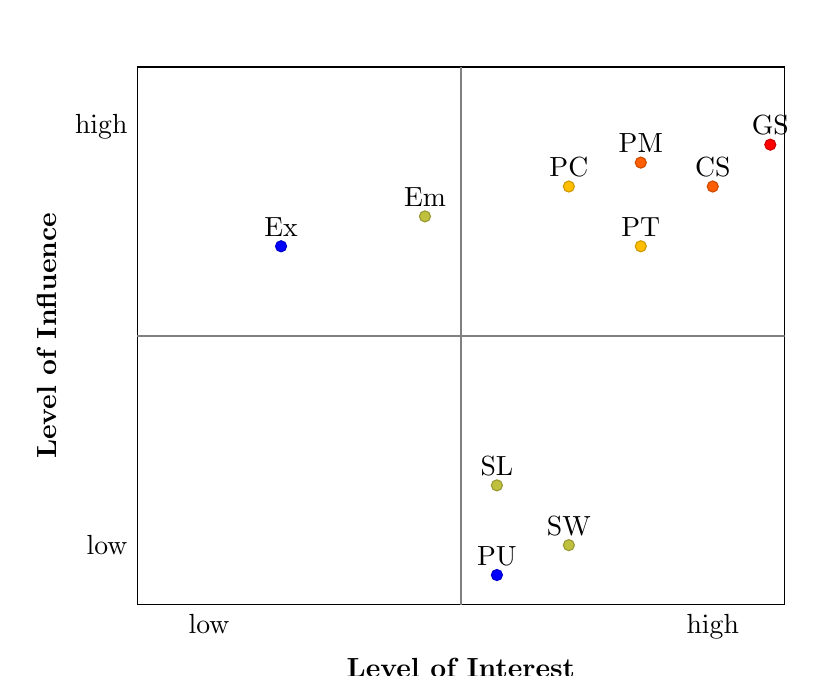
\begin{tikzpicture}
		\begin{axis}[
			scale=1.2,
			xmin=1,
			xmax=10,
			ymin=1,
			ymax=10,
			xtick,
			ytick,
			extra x ticks={2,9},
  			extra x tick labels={low, high},
  			xtick style={draw = none},
  			extra y ticks={2,9},
  			extra y tick labels={low, high},
			ytick style={draw = none},
			xlabel=\textbf{Level of Interest},
			ylabel=\textbf{Level of Influence},
			x
			]
			\addplot[
			scatter,
			only marks,
			nodes near coords*={\myvalue},  
			point meta=\thisrow{color},
			visualization depends on={value \thisrow{myvalue} \as \myvalue},
			] table[x=x, y=y]
			{
			x	y	color	myvalue
			5	7.5	2	Em
			7	2	2	SW
			7	8	3	PC
			3	7	1	Ex
			6	3	2	SL
			9.8	8.7	5	GS 
			8	8.4	4	PM 
			9	8	4	CS 
			8	7	3	PT 
			6	1.5	1	PU
			};
			\addplot[gray,thick, no markers] coordinates {(1,5.5) (10,5.5)};
			\addplot[gray,thick, no markers] coordinates {(5.5,1) (5.5,10)};
		\end{axis}
	\end{tikzpicture}
	\caption{Stakeholder Graph}
	\label{fig:stakeholder}
\end{figure}
\subsection{Internal Stakeholders}\label{ssec:internalStakeholders}
Internal Stakeholders are parties that are a part of the team that is working directly on the project in one way or the other. In this section, the internal stakeholders mentioned in table \ref{tab:stakeholder} will be listed again and explained.

\begin{description}
	\item[Employer] \hfill
	
	The employer in this project is an institution and not a single person. This does not change the fact, that the employer is interested in the project, as he is financing the project. Also the employer could change the outcome, if he is not accepting the proposed plans. It is important, that this party is kept satisfied as more work could be created when the plan has to change.
	\item[Student Workers] \hfill
	
	Student Workers are employed to help in the LOGwear project in general. While they currently are not involved with the process of the creation of the demo facility that might change in the future, therefore they should be kept informed.
	\item[Graduation Student] \hfill
	
	The graduation student is the person mainly responsible for the development of the demo facility and therefore has a lot of responsibility and interest towards the project.
	\item[Project Manager] \hfill
	
	The project manager is responsible for the general planning of the project. Planning meetings with the different parties and coordinating them.
	\item[Company Supervisor] \hfill
	
	The company supervisor is looking over the progress of the graduation student and is giving advice if needed. 
	\item[Project Team] \hfill
	
	The project team are the members of the team actively developing the application prototype and are involved in building the demo facility afterwards.
\end{description}

\subsection{External Stakeholders}\label{ssec:externalStakeholders}
External Stakeholders are parties that are involved in the project, but are not a part of the team actively developing the project. In this section, the external stakeholders mentioned in table \ref{tab:stakeholder} will be listed again and explained.

\begin{description}
	\item[Partner University] \hfill
	
	The partner university is also working on the LOGwear project, but on a different aspect. They might be interested in project of creating a demo facility, but probably will not interfere with it.\\
	
	\item[Pilot Company] \hfill
	
	The pilot company involved is the logistics company KLG. They bring in the highest amount of domain knowledge and are interested in the project to improve their own processes. They could influence the project easily by not approving the planned demo facility due to problems with how the logistics process is modelled.
	\item[Examiner] \hfill
	
	While the examiner is not involved in the project itself, the examiner will finally assesses the performance of the graduation student.
	\item[Supervising Lecturer] \hfill
	
	The supervising lecturer is there to answer questions and support the student from a software engineering standpoint. While not having a lot of influence on the project itself, the supervising lecturer is interested in what the student is doing and especially how he is doing it.
\end{description}

\section{Risks}\label{sec:risks}
Risk management is about identifying risks and finding solutions to problems before they can occur. The list of risks can be found in table \ref{tab:RiskRegister}. The identified risks will increase as the project moves forward. Especially when a decision is made for the wearable and the process. 

\begin{table}[htbp]
\centering
\footnotesize
\resizebox{\textwidth}{!}{
\begin{tabular}{|>{\raggedright\arraybackslash}p{.03\textwidth}|>{\raggedright\arraybackslash}p{.1\textwidth}|>{\raggedright\arraybackslash}p{.2\textwidth}|>{\raggedright\arraybackslash}p{.08\textwidth}|>{\raggedright\arraybackslash}p{.08\textwidth}|>{\raggedright\arraybackslash}p{.15\textwidth}|>{\raggedright\arraybackslash}p{.13\textwidth}|>{\raggedright\arraybackslash}p{.11\textwidth}|}
\hline
\textbf{Nr} & \textbf{Risk Name}                                    & \textbf{Description}                                                                                                      & \textbf{Prob-ability} & \textbf{Impact} & \textbf{Root Cause}                                                                                       & \textbf{Potential Responses}                                              & \textbf{Risk Owner} \\
\hline
1           & Wearable unavailable (W)         & The wearable desired to be used in the demo facility is unavailable.                                                      & Low                  & Medium          & The desired product is a prototype or similar.                                                            & Choosing a different wearable that is already readily available.          & Graduation Student  \\ \hline
2           & Demo Area (D) & A demo area is in mind that could potentially be rented, but that could not be possible.                                  & Medium               & Medium          & The owner of the place does not rent the area.                                                            & Researching possible places where the demo facility could be created.     & Graduation Student  \\ \hline
3           & Unusable wearable (U)             & A wearable is chosen that does not have the capabilities to fulfill the things that were planned with the demo facility.  & Low                  & High            & Too little research done on the wearables, or the researched material was wrong.                          & Altering the demo scenario to accommodate the problems with the wearable. & Graduation Student  \\ \hline
4           & Vocabulary unclear (V)           & The vocabulary used in the logistics branch, especially abbreviations and acronyms might cause problems in communication. & High                 & Low             & The graduation student has too little knowledge of the logistics branch, at the beginning of the project. & Asking questions if a word's or sentence's meaning is not clear.          & Graduation Student \\ \hline
5 & Communi-cation Problems (C) & When explaining a task, a phrase or word is understood differently from different parties. & High & Medium & The proper definition is not known to everyone and are expecting a different meaning from a given phrase or word. & When the misunderstanding is discovered the different parties talk out what is expected from that term and come to a common understanding. & Project Team \\ \hline
\end{tabular}
}
\caption{Risk Register}
\label{tab:RiskRegister}
\end{table}

\begin{figure}[H]
	\centering
	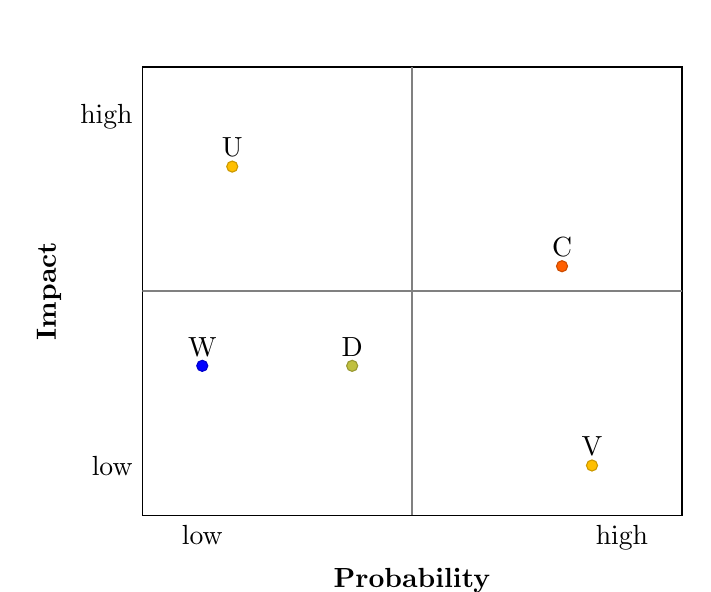
\begin{tikzpicture}
		\begin{axis}[
			scale=1,
			xmin=1,
			xmax=10,
			ymin=1,
			ymax=10,
			xtick,
			ytick,
			extra x ticks={2,9},
  			extra x tick labels={low, high},
  			xtick style={draw = none},
  			extra y ticks={2,9},
  			extra y tick labels={low, high},
			ytick style={draw = none},			
			xlabel=\textbf{Probability},
			ylabel=\textbf{Impact},
			x
			]
			\addplot[
			scatter,
			only marks,
			nodes near coords*={\myvalue},  
			point meta=\thisrow{color},
			visualization depends on={value \thisrow{myvalue} \as \myvalue},
			] table[x=x, y=y]
			{
			x	y	color	myvalue
			2	4	1	W
			4.5	4	2	D
			2.5	8	3	U
			8.5	2	3	V
			8	6	4	C
			0	0 	5
			};
			\addplot[gray,thick, no markers] coordinates {(1,5.5) (10,5.5)};
			\addplot[gray,thick, no markers] coordinates {(5.5,1) (5.5,10)};
		\end{axis}
	\end{tikzpicture}
	\caption{Risk Graph}
	\label{fig:risks}
\end{figure}

In figure \ref{fig:risks} the risks can be seen in a graph that shows their Probability and Impact again. The color emphasizes the amount of attention a risk should get, in order for the project to continue smoothly. The figure also shows more fine grained the probability and impact of the risks than just low, medium and high.

\clearpage

\section{Quality Management}\label{sec:qualityManagement}

Metrics used to determine the quality of the project:

\begin{description}
	\item[Code Coverage] \hfill \\
		Code coverage is a useful metric showing the amount of code covered by unit tests. While they should not be the only way of testing an application of this size, they are still useful to see if a single components works on their own. Due to time constraints code coverage of 100\% is most likely not achievable and a coverage of about 90\% is aimed towards.
	\item[Language Conventions] \hfill \\
		Programming languages usually have conventions on how the semantics of the code should look like to be considered code. These conventions will most likely be followed, and if there are any changes to that they will be listed here.
	\item[Documentation] \hfill \\
		Documentation of a method will include the parameters involved, the return result, usage and general how something works. Furthermore documentation explaining the class and package will be created in a similar fashion. Furthermore created diagrams will be made available and also documented.
	\item[Performance Testing] \hfill \\
		The wearable part of the application might need to be performance tested, as wearables tend to be less powerful than most computing devices normally used. This will be decided when the application is creating problems regarding to performance.
\end{description}

\section{Definition of Done}\label{sec:definitionOfDone}
A part of the software project is done, when it is fully designed, implemented, documented and tested. When that part of the application is passing all of these criteria it is added to a repository where the result is build. When that build is successful that part of the application is done, for the moment. When that part needs to be changed in the future the same procedure will be used again.
\section{Planning}\label{sec:planning}
The initial schedule for the project can be seen in table \ref{tab:schedule}. It is to be mentioned, that the schedule is subject to change as the project goes on. The project will be executed in a scrum-like way that is adapted to the group, given the group size of two developers.
\begin{table}[htbp]
\centering
\large
\resizebox{1\textwidth}{!} {
\begin{tabular}{|c"cc:cccc:cc:ccccccccc:ccc:c|} \hline
\textbf{Sprints} & \multicolumn{2}{>{\centering\arraybackslash} m{.15\textwidth}|}{\textbf{Logistics Processes \& Wearables}} & \multicolumn{4}{>{\centering\arraybackslash} m{.35\textwidth}|}{\textbf{Reference Architecture}} & \multicolumn{2}{>{\centering\arraybackslash} m{.25\textwidth}|}{\textbf{Research Demo Facility}} & \multicolumn{9}{c|}{\textbf{Demo Facility Design and Implementation}}                   & \multicolumn{3}{>{\centering\arraybackslash} m{.25\textwidth}|}{\textbf{Creation Demo Facility}} & \multicolumn{1}{>{\centering\arraybackslash} m{.08\textwidth}|}{\textbf{Buf-fer}} \\ \thickhline
Date                 & 06.02              & 13.02              & 20.02                & 27.02                & 06.03         & 13.03        & 20.03        & 27.03 & 03.04 & 10.04 & 17.04 & 24.04 & 01.05 & 08.05 & 15.05 & 22.05 & 29.05 & 05.06         & 12.06        & 19.06        & 26.06                             \\
Week                       & 6                  & 7                  & 8                    & 9                    & 10            & 11           & 12           & 13    & 14    & 15    & 16    & 17    & 18    & 19    & 20    & 21    & 22    & 23            & 24           & 25           & 26 \\\hline       	              
\end{tabular}
}
\caption{Schedule}
\label{tab:schedule}
\end{table}

The schedule is divided in work packages that are to be executed, it is to be noted, that each work package could be split into multiple sprints in the future. In the following subsections the work packages will be explained.

\subsection{Logistics Processes \& Wearables}
This work package includes research about the gives processes and wearables in general, as well as already choosing potential wearables that could be used to improve the process. The end result for this should be a decision on process and wearable. But the result for this could potentially take longer than this task is scheduled. The wearables should be ranked after getting hands-on experience on them, therefore some of them have to be ordered first.

\subsection{Reference Architecture}
A reference architecture should be created for a sample wearable application. What this work package contains is, the creation of diagrams which show the communication from a wearable to the \gls{wms} or something similar. What should not be created is a full reference architecture for a process that is implemented with a concrete wearable. 

It is about creating the always needed layers when using a wearable in a way that supports most wearable solutions.

\subsection{Research Demo Facility}
This task includes researching what physical objects and what systems would be needed to create a demo facility that could showcase a single process with a single wearable. This also includes the gathering of knowledge of where the demo facility should be created and where to get the needed objects.

\subsection{Demo Facility Design and Implementation}
The work package includes the creation of the software design and implementation for the wearable and all aspects that are needed to fully showcase a process.

\subsection{Creation Demo Facility}
This task includes the physical creation of the demo facility. This means setting up shelves with packages to scan and put on a hand pallet truck. Setting up barcodes on the packages to scan. Setting up an environment that can showcase what is happening better to an audience.

\section{Research}
\begin{frame}\frametitle{Research}
	\begin{itemize}
		\item 1
	\end{itemize}
\end{frame}
\chapter{Reference Model}\label{cha:reference}
The \gls{reference model} of the LOGwear project is a model that shows how the communication from a wearable to the \gls{wms} or some other system might work. This does not mean that every communication necessarily needs to be implemented like displayed in the \gls{reference model}, but that in general every wearable is able to communicate with an underlying system in the way it is displayed.
The model can be seen in figure \ref{fig:referenceModel}.
\begin{figure}[htbp]
	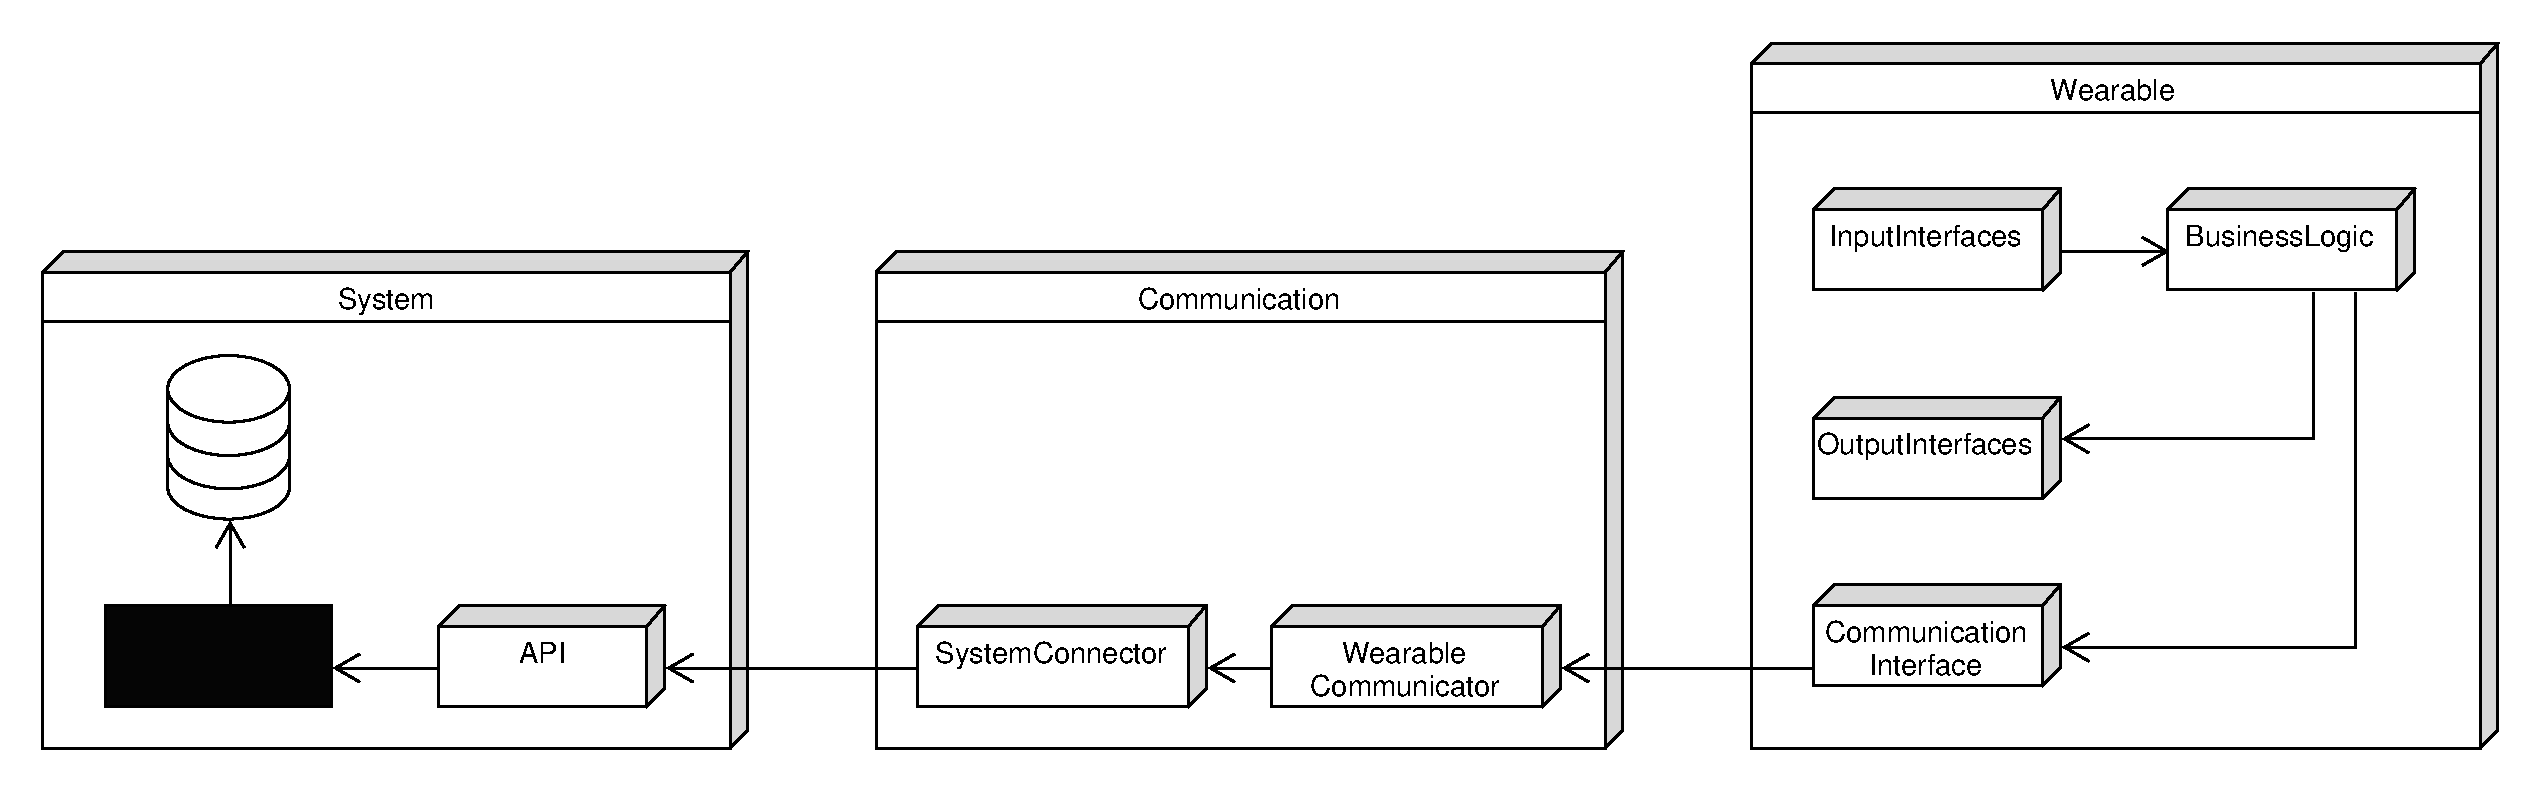
\includegraphics[width=\linewidth]{images/PackageModel_ReferenceArchitecture}
	\caption{Reference Model LOGwear}
	\label{fig:referenceModel}
\end{figure}

\section{Definition}
A \gls{reference model} is an abstract design used to help others understand the general concept and the relationships between existing entities of a specified environment. Furthermore a \gls{reference model}, in general, does not model anything with a specific technology in mind and rather models everything as general as possible. This is done so that when creating an architecture around the \gls{reference model}. The \gls{reference model} can be used as a template to start working with. Not as a constraint, that holds the architects back. When implementing the \gls{reference model} with a specific technology, it is needed to change existing parts or add new parts to fit the given constraints. A \gls{reference model} as is, is not directly implementable due to the abstract nature.

The aim for a \gls{reference model} is to standardize the way how developers in the future implements an application in the given domain, regardless of the used technologies.\citep{website:oasis-rm}

\section{Requirements}
The reference model is an abstract construct, therefore the functional requirements towards it are taken as example to prove the validity of the model. The functional requirements are listed in the form of use cases The non-functional requirements are towards the model itself and not towards an implementation of it. 

\subsection{Functional Requirements}
The functional requirements represents example cases that should be possible to implement with the reference model. The cases that will be given do not need to be fulfilled all at once, but all of them should be possible with the reference model. Given in the following list are short descriptions of the use cases, while the full use cases themselves can be seen in the appendix, section \ref{sec:useCasesReferenceModel}. The example cases given here are based on the demo scenario chosen, but more use cases can be defined for different scenarios.

\begin{description}
	\item[Get Order] \hfill \\
		An order document is fetched and in some way displayed to the worker.
	\item[Order Confirmation] \hfill \\
		The order the worker is currently working on is being worked on and the parts of the order is being confirmed. When all parts of the order are finished the whole order can be confirmed.
	\item[Order Control] \hfill \\	
		When an order is being picked, the wearable is supporting the worker in counting the right number of parcels and picking the correct article in the first place.
\end{description}


\subsection{Non-Functional Requirements}
The non-functional requirements towards the reference model are the most important details that were taken in consideration when the reference model was designed. They can be seen in the following list:

\begin{description}
	\item[Documentation] \hfill \\
		The reference model needs to be properly documented. The advantages and disadvantages of the design need to be properly explained to a person that potentially wants to implement a system based on it.
	\item[Extensibility] \hfill \\
		The reference model needs to be extensible since some companies might have some more requirements towards their system than is intended for a general case. Adding functionality to the reference model should be possible.
	\item[Modifiability] \hfill \\
		The existing ideas of the reference model should be modifiable. Companies are going to use different wearables and infrastructure, and the reference model should be adjustable to fit a lot of possibilities without the need to create a completely new system architecture.
\end{description}

\section{Design}
As can be seen in figure \ref{fig:referenceModel} the \gls{reference model} is divided into three different packages that all fulfil different responsibilities. First it will be described what this \gls{reference model} can help to create. Therefore the general thought behind the whole model will be explained and afterwards the three packages \texttt{system}, \texttt{communication} and \texttt{wearable} will be explained on their own.

The concept is simple, a wearable is connected to a communication layer, that then again connects to a system, that could be anything, as long as it has an \gls{api}. The arrows are not indicating an information flow but rather an instruction flow. The box that the arrow leaves does invoke an instruction in the box that the arrow points to. The sources of information are generally the \texttt{InputInterfaces}, and the incoming information is spread from there. Depending on the incoming information, actions are invoked. 

The \gls{reference model} is purposely minimalistically designed, to allow most infrastructures and wearables, to apply the model, with as few changes as possible. If for example a new \gls{wms} was used the only component that needs to be changed is the \texttt{SystemConnector} in the \texttt{communication} package. In that case, the wearable that are in use, can also continue to work, just like they normally would, without the need for a new version to be deployed on all of them.

\subsection{Wearable}
The \texttt{\gls{wearable}} package is representing the actual physical wearable, or a set of wearables, that a worker is using. This could be either \gls{smartglasses}, \gls{smartwatch}es, a ring-scanner or some other \gls{wearable}. It could also be a combination of wearables that is used in order to fulfil a certain task. In such cases it is still possible to stick to the \gls{reference model} either by changing the existing model, with multiple \texttt{BusinessLogic} classes in the different wearable and a manager that could handle that. Or it could be, that even when using multiple wearables at once, a single wearable is handling the business logic of all wearables. Then the other wearables could be addressed by just their input- and output- interfaces.

Further on the wearable package is again held as simple as possible. The \texttt{InputInterfaces} are there to get information from the outside world and the \texttt{OutputInterfaces} are there to somehow represent information to the outside world. The \texttt{BusinessLogic} is there to process the incoming data and invoke the appropriate actions, that could be either displaying some information to the user or making a call to the underlying system through the \texttt{CommunicationInterface}.

The \texttt{CommuncationInterface} is the means of communication with an outside computer source, this could be radio, bluetooth, \gls{rest} via \gls{wlan} or some other way of communication. The \texttt{WearableCommunicator} in the \texttt{Communication} package just needs to be able to receive and understand the messages.
\subsection{Communication}\label{subsec:communication}
The \texttt{communication} package is existing due to the different technologies used from \gls{wearable}s to connect to other computing devices. The communication layer might also be the only place, where information can be fully controlled by the developer, this is especially interesting when the \texttt{system} is controlled by a third-party. Also needed actions can be taken, if the incoming data has to be transformed into a different format, before either the \texttt{\gls{api}} or the \texttt{wearable} can understand it. 

The \texttt{communication} package could potentially be removed, if the wearable has the needed technology in place to directly connect to the \gls{api} of the given system. But this is in general not recommended, as the communication layer allows the developer to create a more standardized flow of information.

\subsection{System}
The \texttt{system} package here can be something like a \gls{wms} of the company. A system that is mostly a black box with an \gls{api} and a database. Most of the time, the \texttt{system} cannot be changed by the developer, therefore the developer needs to use the possible ways to connect to the given \gls{api}.

\section{Variations}
Multiple variations can be made to the reference model and some of the most likely variations of the reference model will be listed in this section.

\subsection{No Communication Layer}
As already mentioned in subsection \ref{subsec:communication} about the communication layer, the communication layer might be skipped in situations where the wearable is able to directly connect to the \gls{wms}. How the model changes in such situations can be seen in figure \ref{fig:referenceModel_NoCommunication}. 

\begin{figure}[htbp]
	\begin{center}	
	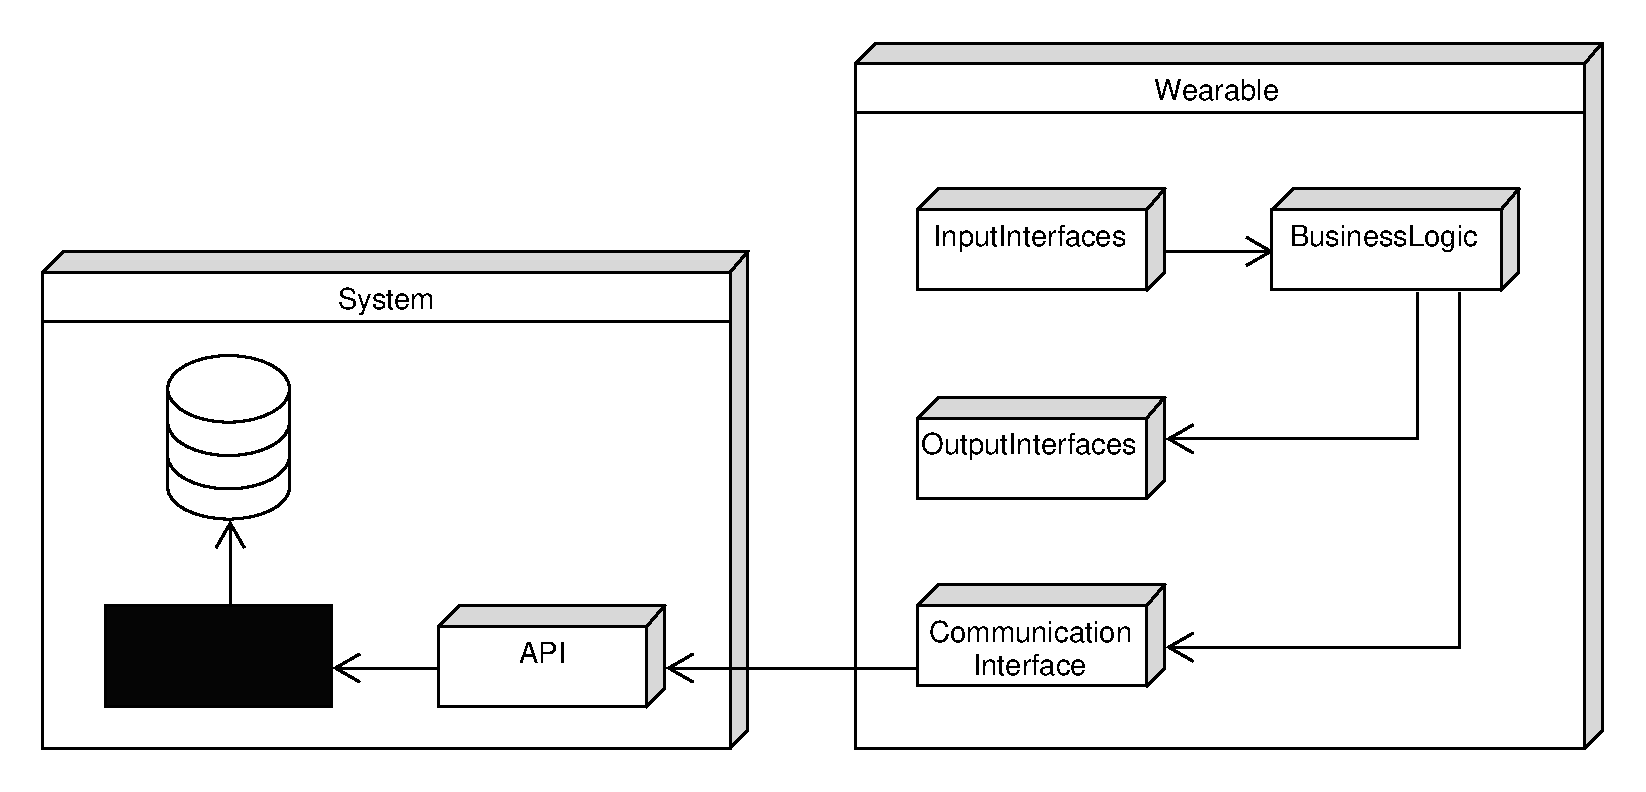
\includegraphics[width=\linewidth]{images/PackageModel_ReferenceArchitecture_NoCommunication}	
	\end{center}
	\caption{Reference Model - No Communication Layer}
	\label{fig:referenceModel_NoCommunication}
\end{figure}

Apart from the removal of the communication layer the reference model still works exactly the same. This change is rather likely since a lot of newer wearables are able to connect to a rest interface or something similar.

\subsection{Push Messages}
The possibility to send \gls{pushmessage}s is also a very likely addition to the existing reference model. An example case for the usefulness of this is, an urgent order is coming in and a coordinator wants to see which person might be the most responsible for that order. Afterwards the coordinator can just contact the worker through his wearable and give him the new order directly through a push message. A possible configuration for this can be seen in figure \ref{fig:referenceModel_PushMessages}.
\clearpage

\begin{figure}[htbp]
	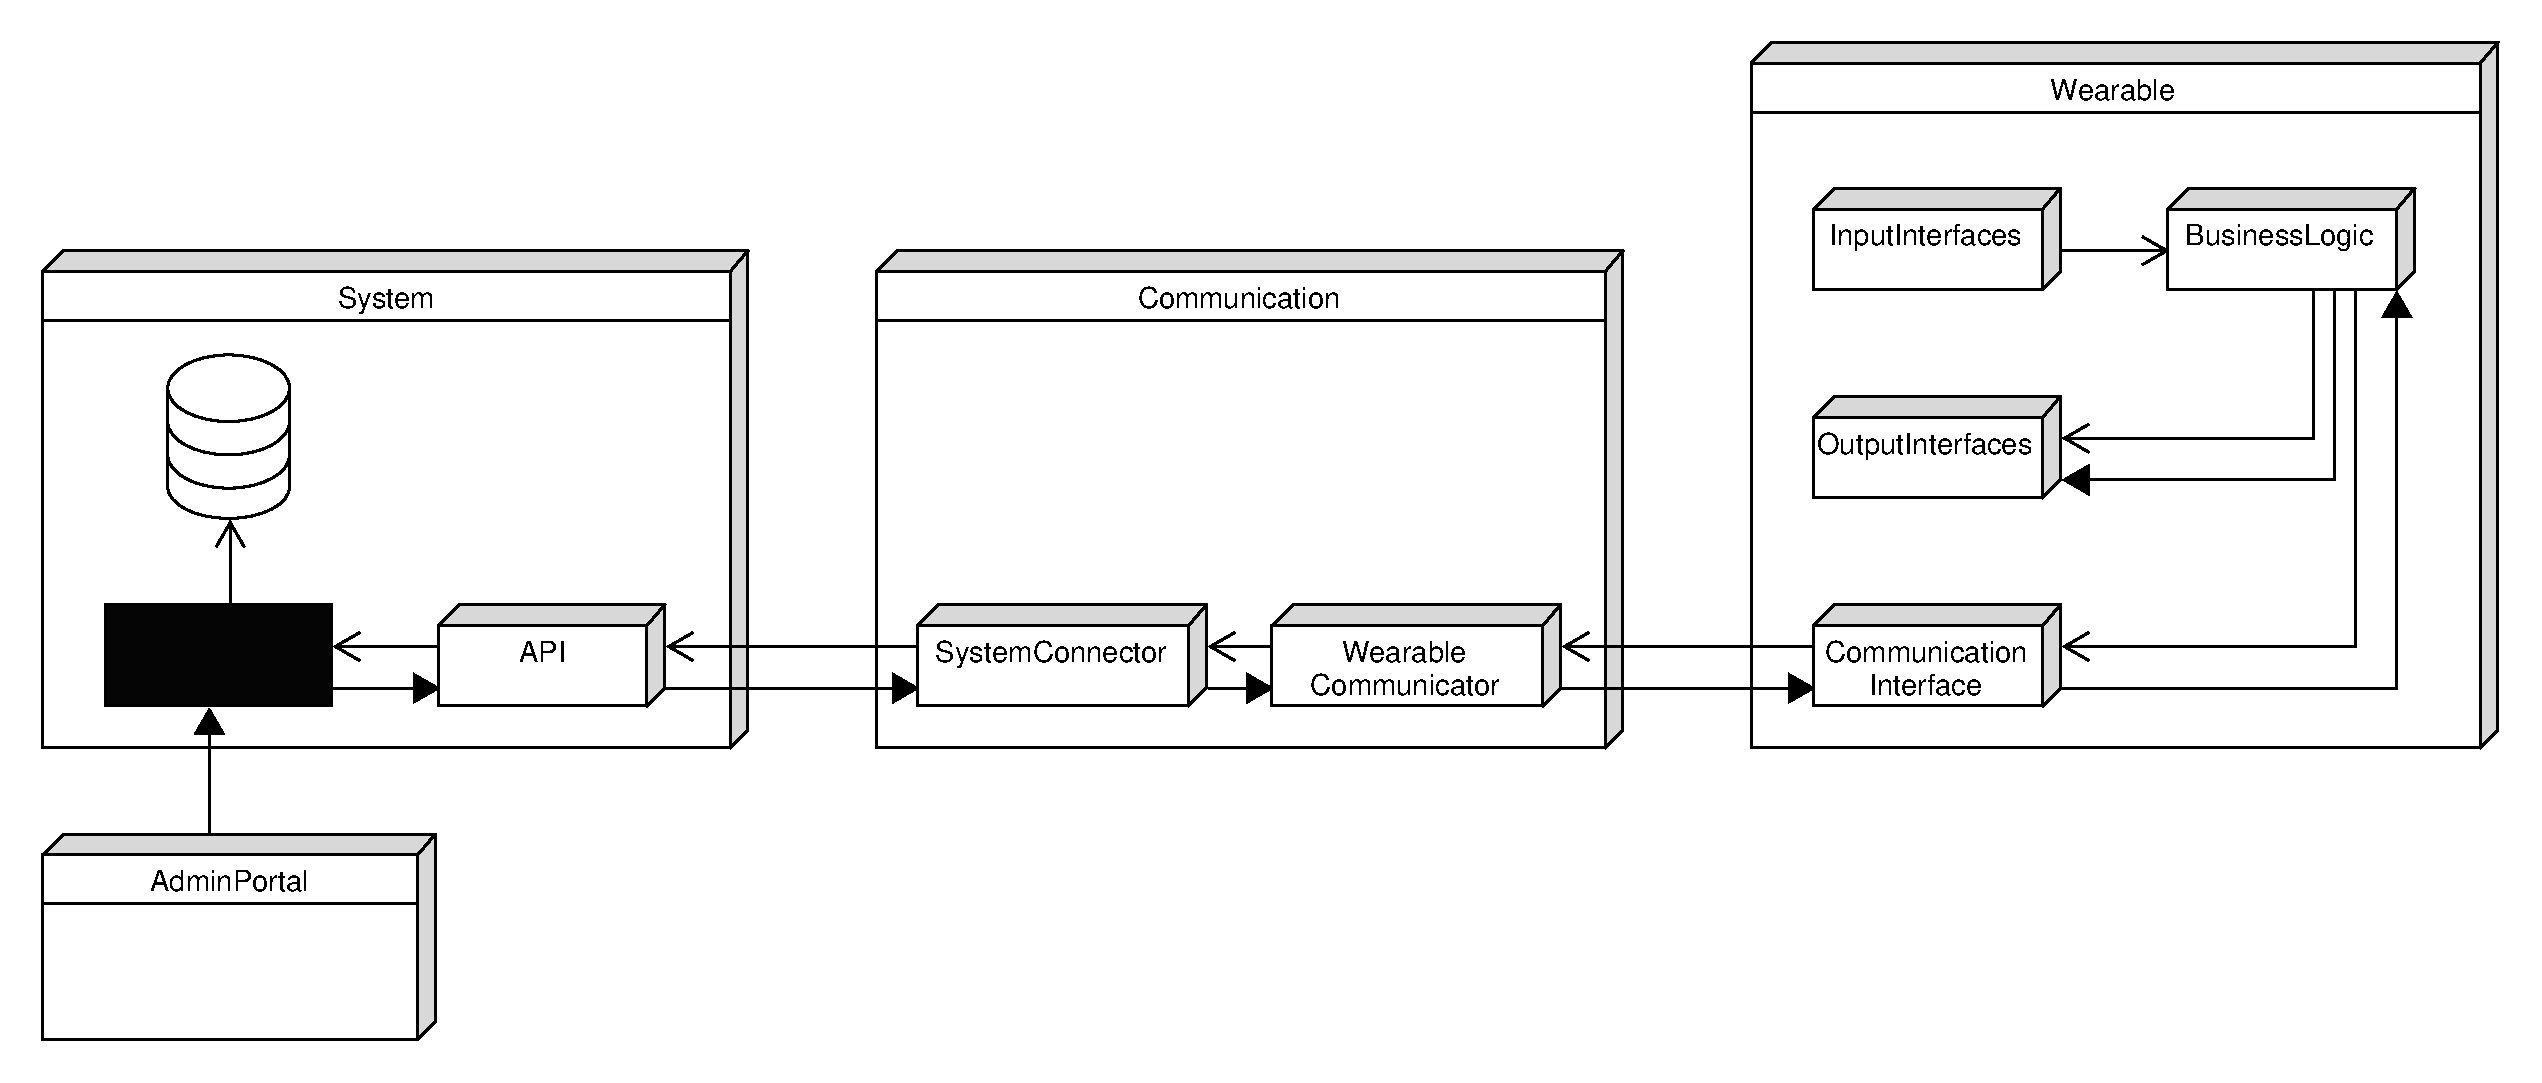
\includegraphics[width=\linewidth]{images/PackageModel_ReferenceArchitecture_PushMessages}
	\caption{Reference Model - Push Messages}
	\label{fig:referenceModel_PushMessages}
\end{figure}

Like in the normal reference model, the normal arrows show an instruction flow that is originating from the worker. The arrows with the filled arrow head are the instruction flow from the coordinator and therefore the push messages. The AdminPortal is added here as a possibility for a coordinator to check on the state of current orders and what workers are currently most occupied. This helps the coordinator choose a worker that is available and used to the customer that order something and is a higher priority.

\subsection{Web Application}
Another likely variation of the reference model is a scenario in which a web application is replacing the communication layer. This reduces the load on the wearable and allows a more uniform handling of multiple wearables. This variation of the reference model can be seen in figure \ref{fig:referenceModel_WebApp}.

\begin{figure}[htbp]
	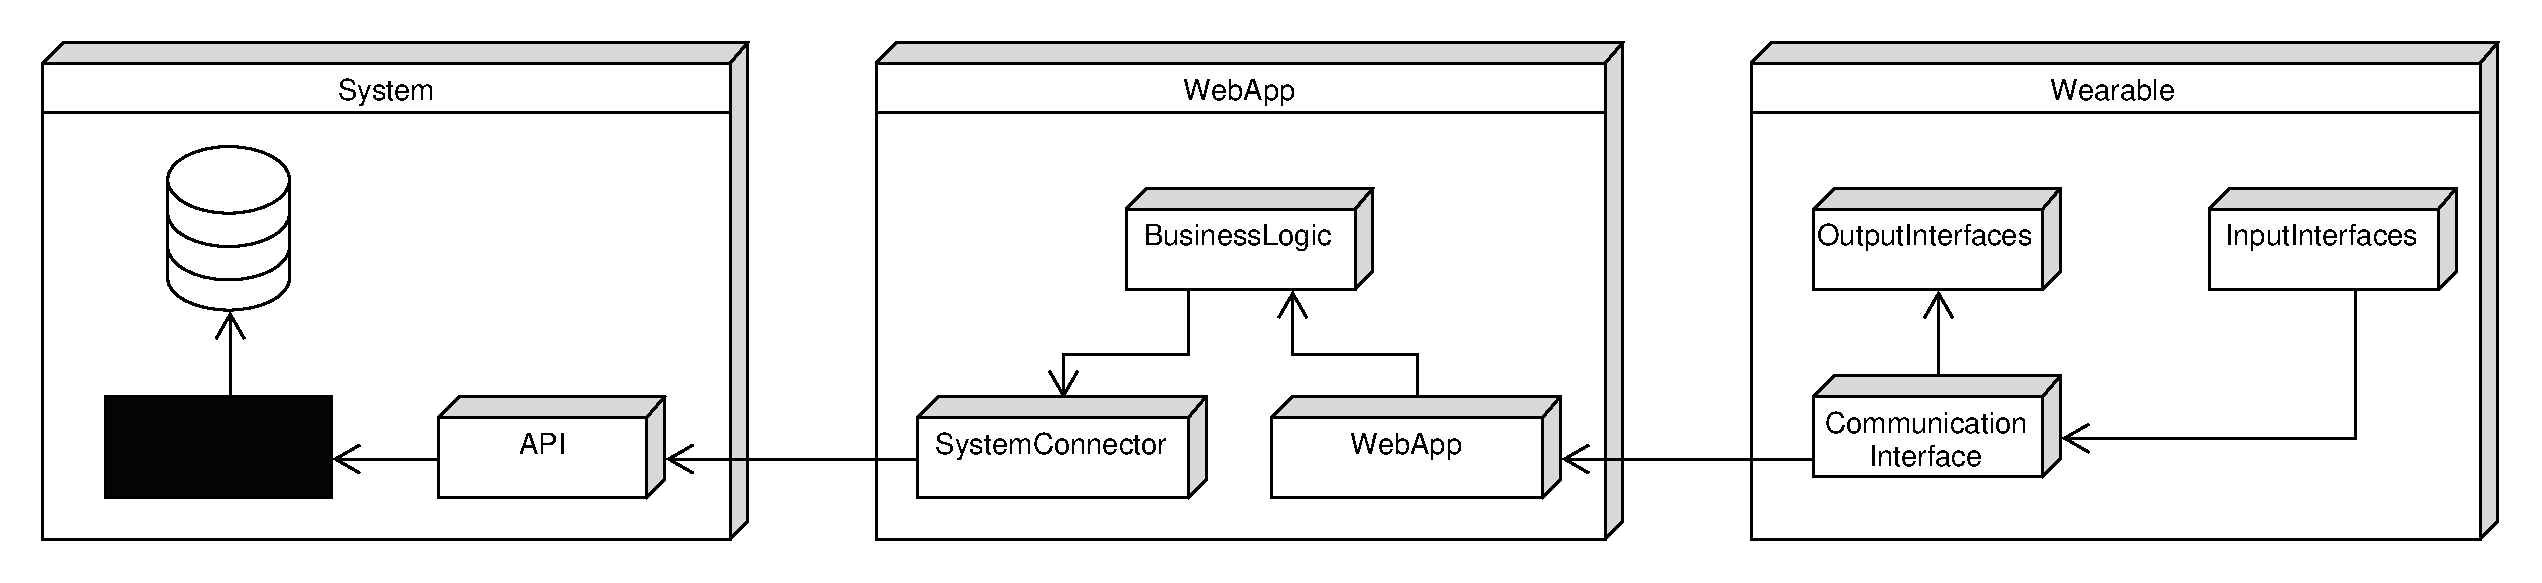
\includegraphics[width=\linewidth]{images/PackageModel_ReferenceArchitecture_WebApp}
	\caption{Reference Model - Web Application}
	\label{fig:referenceModel_WebApp}
\end{figure}

The \texttt{WebApp} package here is just held as simple here, since the way to implement a web application can vary a lot. If a web application is implemented using the \gls{mvvm} patter, \gls{mvc} pattern, \gls{mvp} pattern or some other pattern to implement web applications, is not relevant for the model and is therefore ignored here. The other parts of the reference model are mostly similar, the business logic is moved from the wearable to the web application. This is done to reduce the load on the wearable, which might be a problem for some wearables.

\clearpage
\section{Problems}
The main problem that occurred during the creation of the \gls{reference model} was a problem in communication, regarding the names of \gls{reference model} and \gls{reference architecture}. The initial task was understood to create a general-purpose \gls{reference architecture}, that would connect a \gls{wearable} to some kind of system. During the process of creating the different diagrams for the reference architecture and trying to validate them using code. The problem became obvious that trying to go deeper than the now given \gls{reference model}, as seen in figure \ref{fig:referenceModel}, was impossible to do for a general-purpose implementation.

This is the case because of the nature of the given problem. Being able to use any wearable with any system, for any task. Given that two wearables might have completely different sets of input- and outputinterfaces those could not be defined. The communication interface could be different, which leads to being unable to define a communication standard, while the possibility of any task gives no single action that will always be the same.
\chapter{Demo Facility}\label{cha:demoFacility}
Physical creation of the demo facility that showcases the possibilities of the chosen wearable in the process of order picking in a warehouse. As the demo facility is not yet existing the implementation cannot be discussed and explained here, this chapter will therefore focus on the planned infrastructure, the existing design and what is planned for the demo facility in the future. 

There is also a major difference between the demo facility task that will be explained in this report and the task given in the logwear website. \citep{website:logwear} The task that will be executed here will be creating a demo facility in a physical \gls{sandbox} environment and the task explained in the work package on the logwear homepage is about implementing the improved process, using a wearable, at a pilot company and observing the results.

\section{Infrastructure}
The infrastructure of the demo facility is divided into multiple areas:
\begin{description}
	\item[Mock WMS] \hfill \\
		A mock \gls{wms} that allows to store different orders and edit them to have a more realistic demo. While not all functionality has to given, the data has to be persistent and easily resettable to allow showcasing a demo case multiple times. The mock \gls{wms} is living on an azure server and is a \gls{mssql} database.
	\item[Rest API] \hfill \\
		A \gls{rest} \gls{api} that is used to connect to the mock \gls{wms} from an outside perspective, in this case from the communication layer, see subsection \ref{subsec:communication}.
	\item[Communication Layer] \hfill \\
		The communication layer will be living on a server with a connection to the \gls{db} \gls{api} and a connection to the wearable.
	\item[Wearable] \hfill \\
		The wearable will need to connect to the communication layer and process input and output.
\end{description}

The mock \gls{wms} and the \gls{rest} \gls{api} are insignificant parts of the implementation, therefore not a lot of thought was put into the decision on choosing these technologies was done out of curiosity for these technologies or being the most comfortable with them respectively.

\section{Demo Scenario}\label{sec:demoScenario}
The demo scenario explains the process that will be executed during the demo facility. Therefore describing the actions taken in detail, but ignoring how they will be executed, e.g. with or without a wearable. The original process can be seen in the appendix, figure \ref{fig:orderPickingProcessDiagram}. For the actual scenario for the demo facility an activity diagram was created, that can be seen in figure \ref{fig:activityDemoScenario}. 

\begin{figure}[htbp]
	\begin{center}
	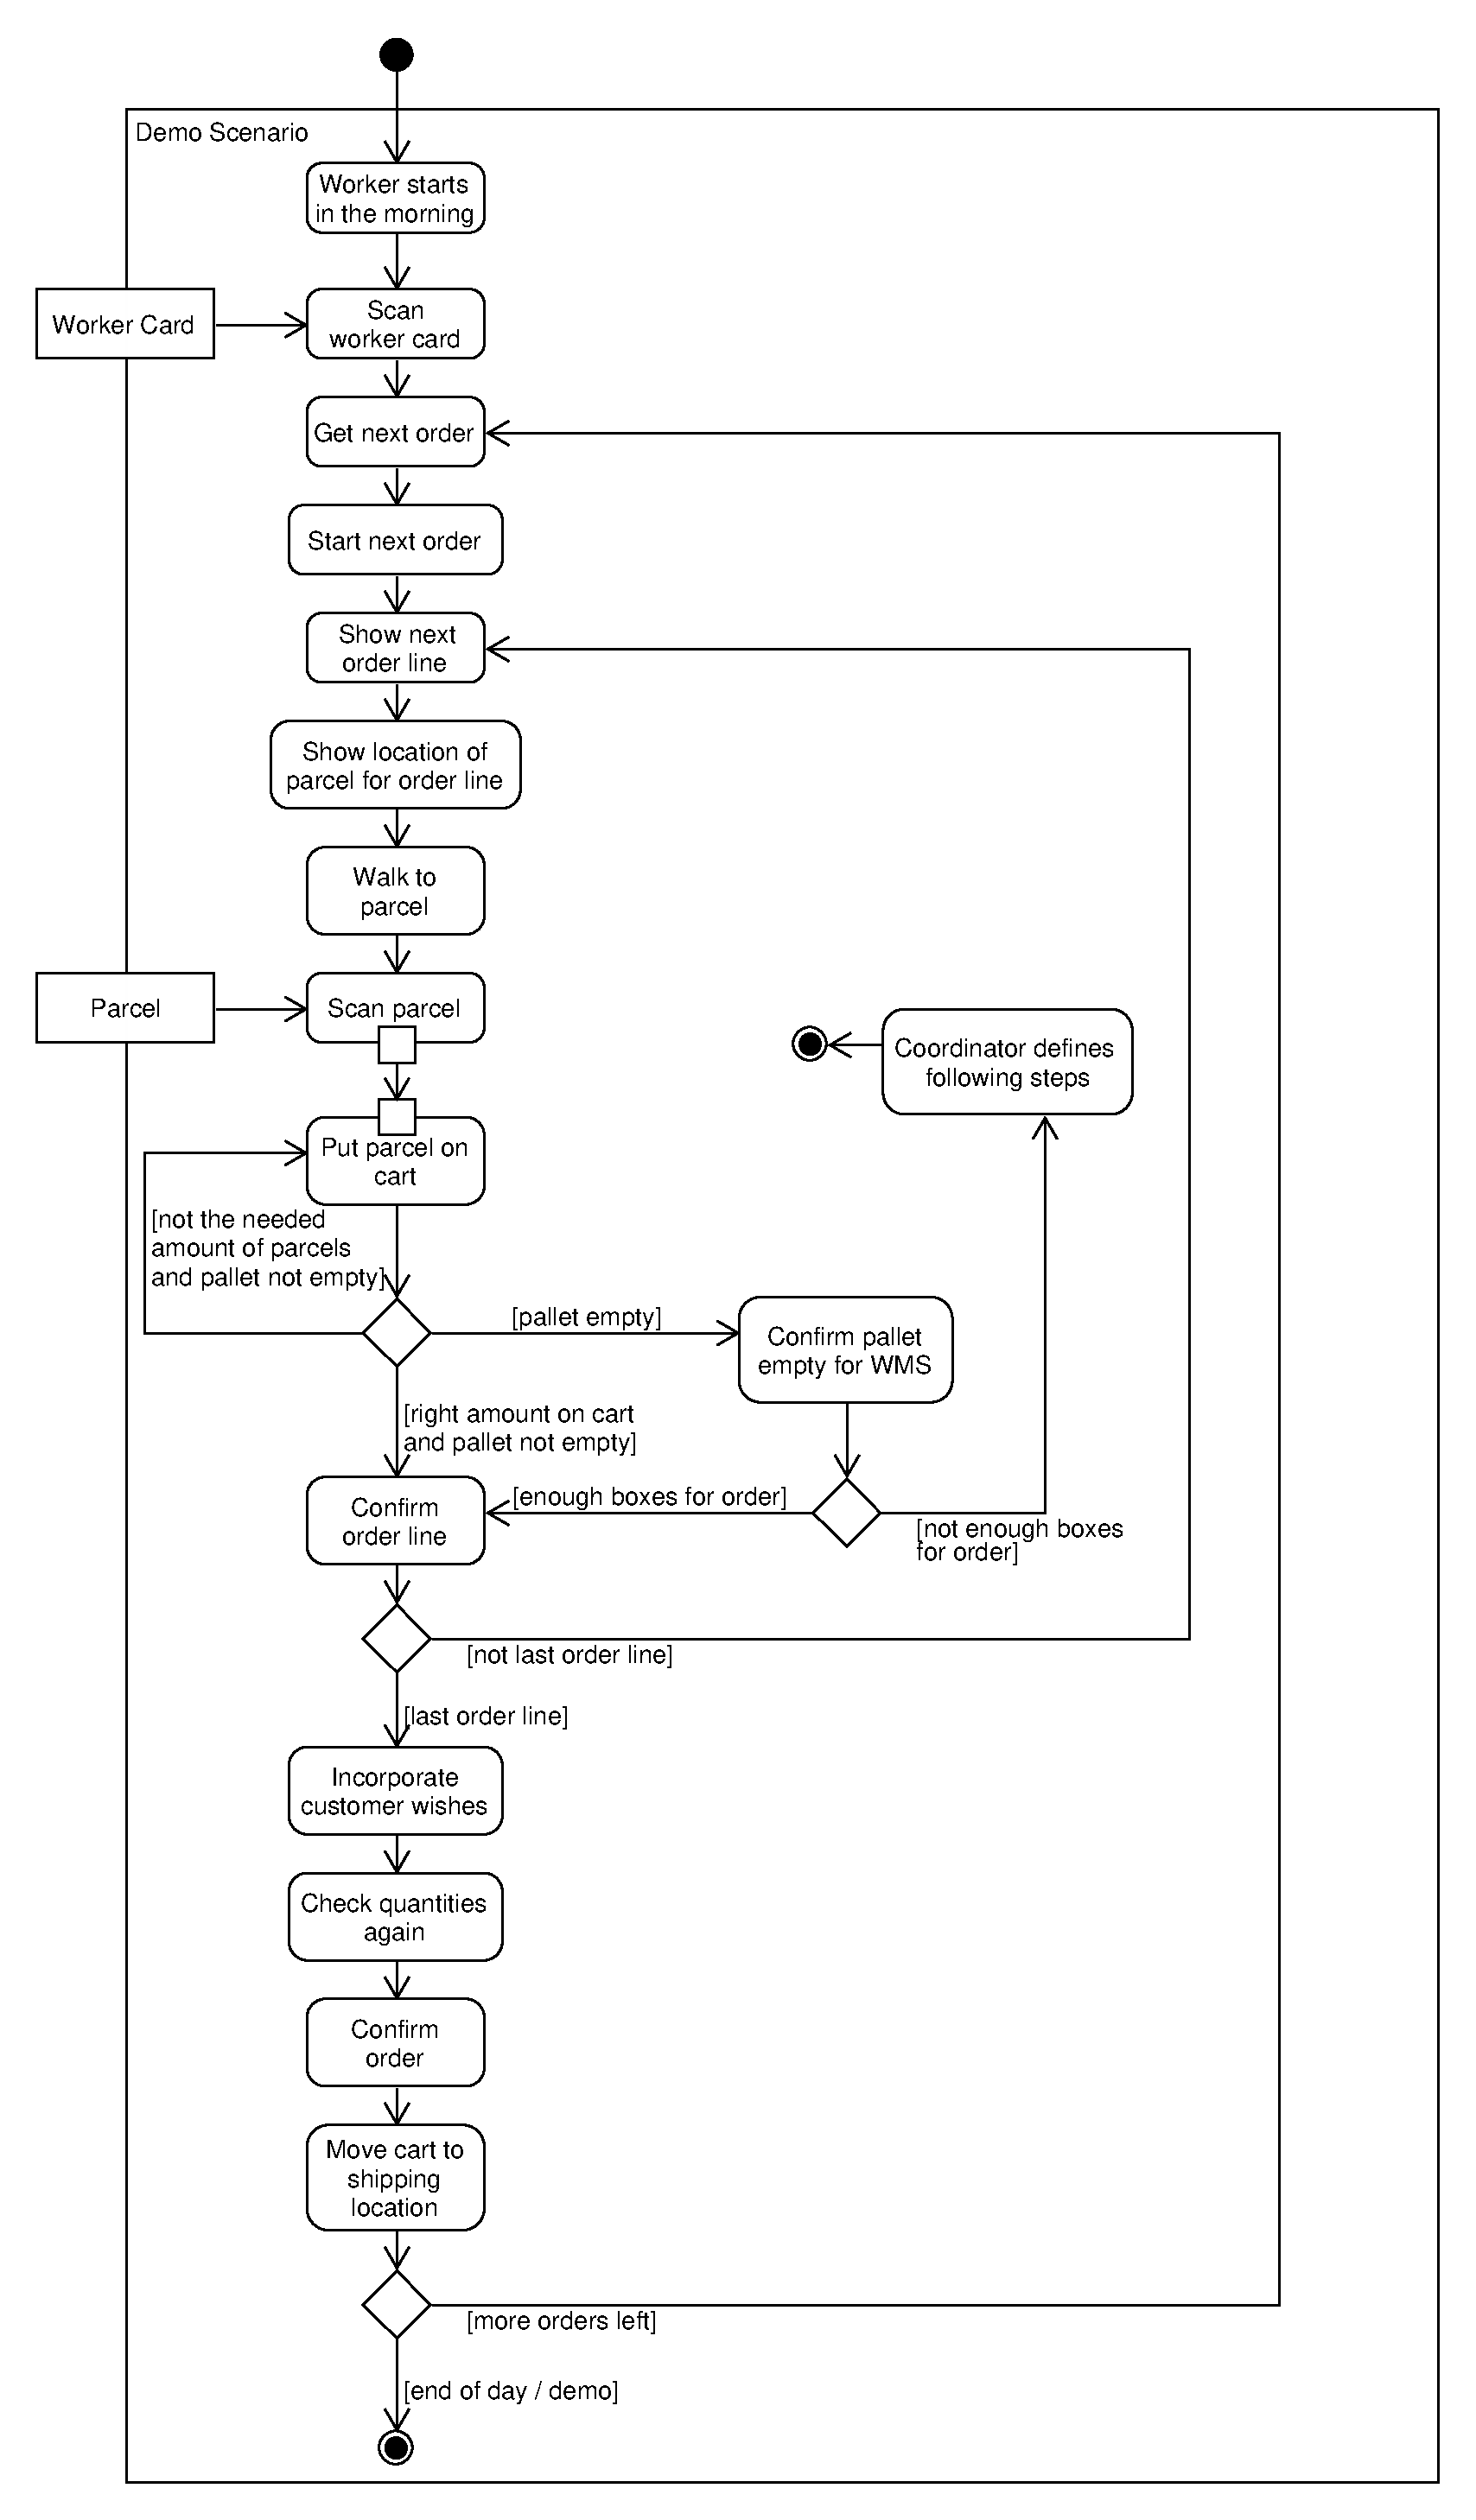
\includegraphics[height=\textheight]{images/activityDiagram_demoScenarioNoExceptions}
	\end{center}	
	\caption{Activity Diagram Demo Scenario}
	\label{fig:activityDemoScenario}
\end{figure}

\cleardoublepage

This diagram was created for multiple reasons:

\begin{description}
	\item[Readability] \hfill \\
	The scale of the original process diagram made it hard to process. One goal was to create a more compact diagram.
	\item[Purpose] \hfill \\
	The original diagram had a different purpose, it was supposed to model the process of one of the pilot companies in its entirety. The purpose of the activity diagram is to model a demo case, that does not need to show every single detail of the process in the first place.
	\item[Focus point] \hfill \\
	The demo scenario focuses on the general tasks an order picking worker is doing, but is just focussing on the main points for this. The original diagram also includes the connections to the database and also includes tasks outside of the actual order picking.
\end{description}

\textcolor{red}{add description of model}

\section{Design}
The general design for the demo facility application will be based on the reference model described in chapter \ref{cha:reference}. But in the following sections the demo facility specific design will be elaborated further.


\subsection{WMS}
The \acrlong{wms} consists of two parts, the database that is going to contain the data for the demo facility and the database connector. This also defines the interface, with which to connect to the \gls{wms}.

\subsubsection{Database}

Figure \ref{fig:LogicalModelWMS} shows the relations and fields in the database. It can be seen that the database just contains a small amount of information, due to being a demo, an actual \gls{wms} would contain a lot more data. The most important item in the model is the order, as that is the key piece, where most relations lead together. An order has a number that is connecting it to one or multiple workers that are working on them. Furthermore an order consists of multiple \texttt{OrderLine}s. An \texttt{OrderLine} is describing the different lines that would appear on an order, that specify the item and the amount for an order. For a warehouse it is also important to add the pallet where to find the item and if the current line is already acknowledged or not. A pallet has a location in the warehouse and how much of that item are still available in the warehouse. The article corresponds to a name for the article number. Finally an order is ordered by a customer, a customer might have additional wishes for their orders and an address where that customer wants things delivered to.

\begin{figure}[H]
	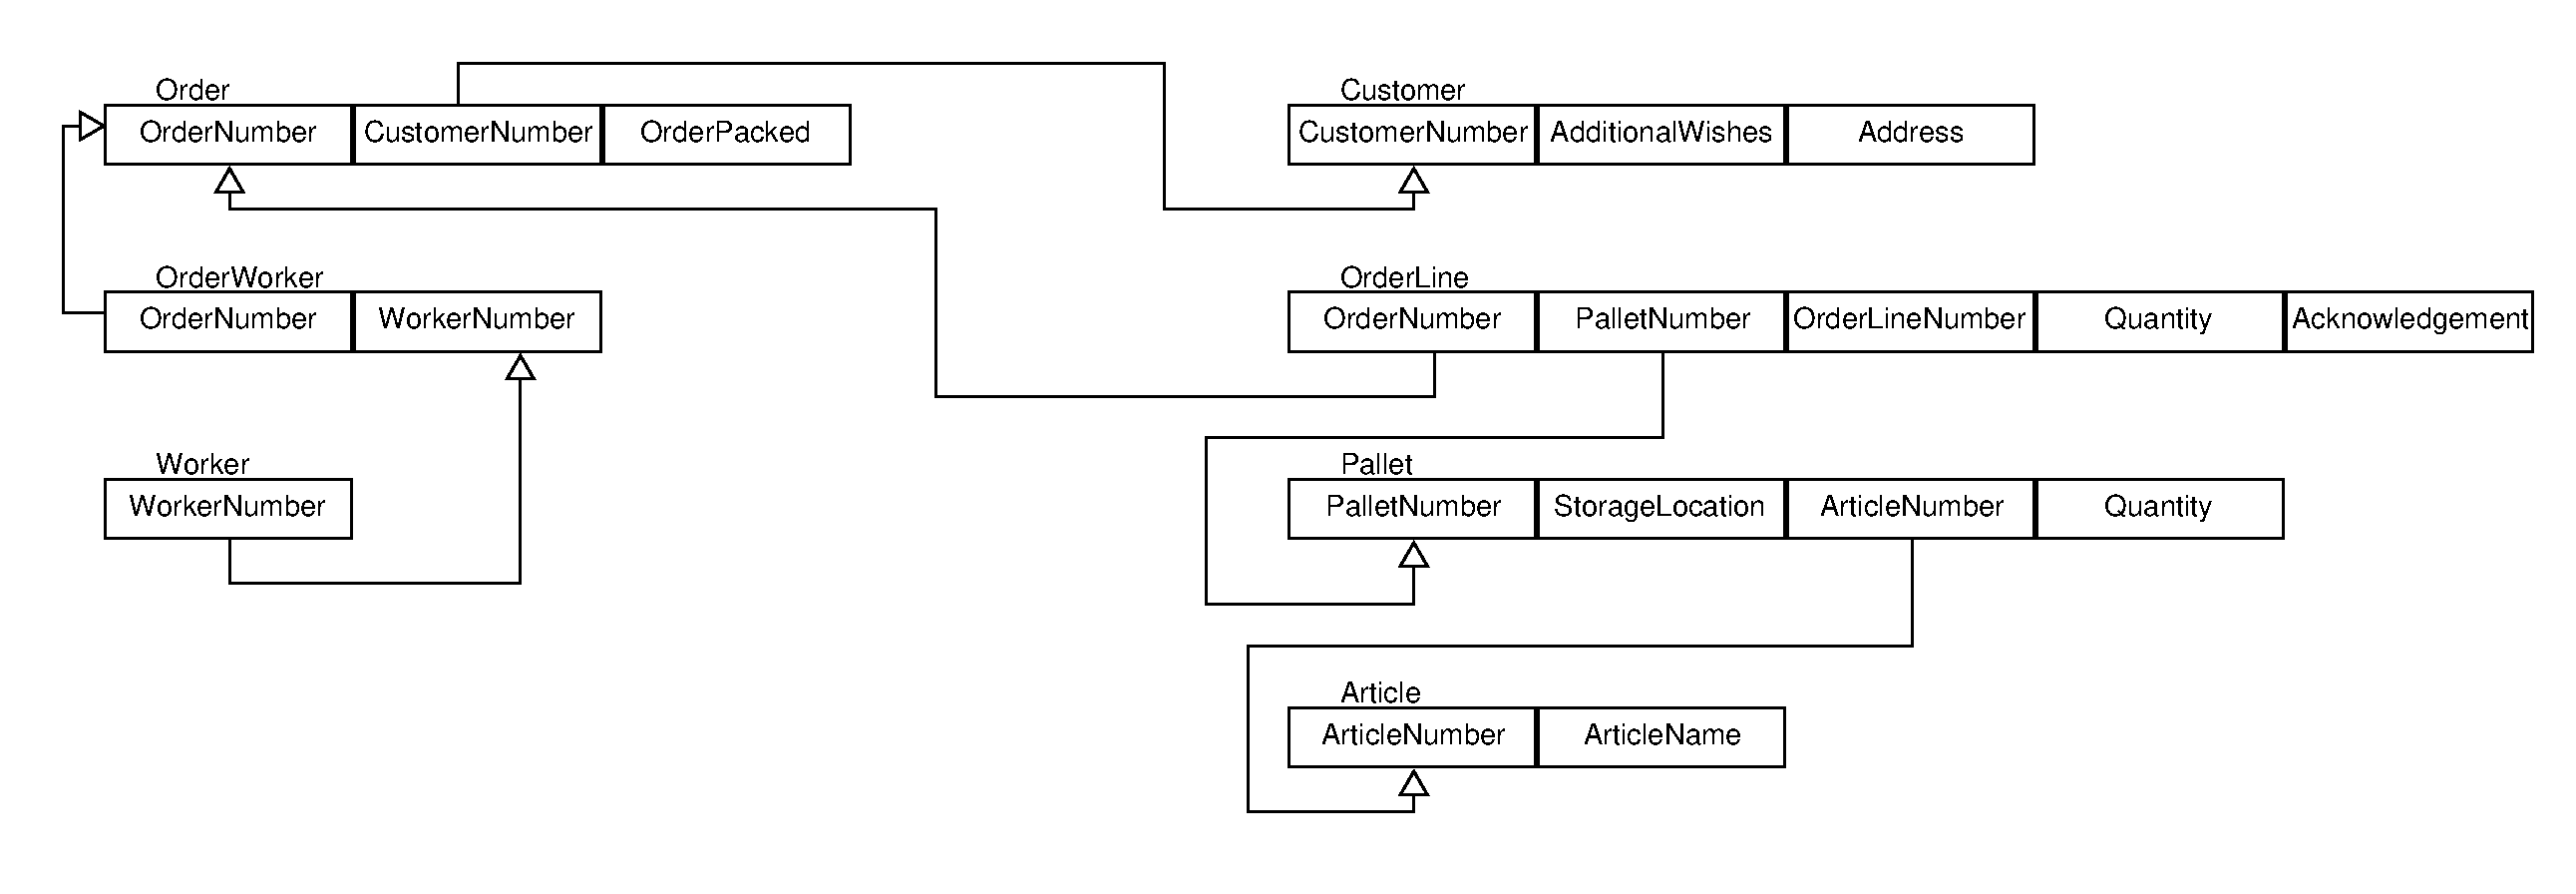
\includegraphics[width=\textwidth]{images/LogicalModel_MockWMS}
	\caption{Relational Schema Warehouse Database}
	\label{fig:LogicalModelWMS}
\end{figure}

For an actual warehouse the customers attributes would change completely, as companies might have multiple addresses, therefore that might change for every order of that customer, making it easier to add an address field to the order and not the customer.  Also a customer might want to add additional wishes just to a specific order or dependent on what might be ordered, therefore the additional wishes might also be moved to the order, but for a demo case, that is not executed at a pilot company, the model is sufficient.

\subsubsection{Interface}
The interface, that is exposed by the \gls{wms}, is a \gls{rest} interface, for the demo case this means that the communication layer, explained in subsection \ref{subsec:communication}, can be skipped, as the wearable chosen in section \ref{sec:processes} is able to connect to a \gls{rest} \gls{api} directly. And for a demo case the communication layer is also not needed to further transform or do similar things with the data that is passing through it. The options available through the \gls{rest} interface are the following:
\begin{description}
	\item[] \hfill \\
	\item[] \hfill \\
	\item[] \hfill \\
	\item[] \hfill \\
\end{description}


\textcolor{red}{Add information about database design, and rest api interfaces}


\subsection{Wearable | Application}
\textcolor{red}{Add information on how the wearable application works, maybe with web interface or direct implementation}

\textcolor{red}{add more sophisticated class diagram}

\section{Planning}
In the future for this task, there will be multiple wearables tried out and then decided which wearable will be used for the demo facility, as described in section \ref{sec:wearables}. Afterwards an application will be written for that wearable, to improve the process chosen in \ref{sec:processes}. 

This application will at least include the functionalities to:
\begin{itemize}
	\item Divide a given room in multiple sectors, to address a single part of the room with a given location string.
	\item Reset the case to allow multiple showcases of the demo.
	\item Allow scanning of \gls{id}s on \gls{parcel}s and pallets.
	\item Send confirmations to the \gls{wms}, that an action has been completed.
\end{itemize}

For the demo environment, an area will be rented that allows to place a rack in there with \gls{parcel}s. The \gls{parcel}s will be equipped with an \gls{id} that can be scanned with the chosen wearable.

When the implementation of the demo application is finished a second one could be started to show \gls{sme} the differences between the possibilities different wearables give the user.

\chapter{Conclusion}\label{cha:conclusion}
Up to this point, the reference model has been fully designed and is documented with multiple variations for different situations. The database for the demo has been deployed on an azure cloud service. The \gls{rest} interface to that database is deployed on the same azure instance. The web application is still being developed at this point, as well as the connection from the wearable to this web application. The facility area has also not been rented and filled at this point. 

Concluding the whole tasks that are to be finished at the end of this project is, that the research process for the available wearables is finished, but more wearables are going to be available in the future for the logwear project. Those wearables will be tested and compared in the future, but that will most likely not be a part of this project anymore. The requirements analysis and design phase for the reference model and the demo facility are also completely finished at this point. The infrastructure surrounding the demo facility is fully implemented as well. The two parts that are not fully implemented at this point are the web application and the wearable application itself. While there are still tasks to complete when that is finished as well, these are the main tasks that are a part of this project.



%The reference model is the only current deliverable really created up to this point. This is due to the reference model being a crucial point of the research project. As the research goes on the reference model will be used as the artifact that is used to show developers on how a wearable system should look like in a logistics environment. Therefore the design went through multiple iterations to allow it to fit as many use-cases as possible, while reducing the need to change a lot of the design for each use-case.

%The design of the reference model, even though a few communicational problems arose with what was actually expected from it, was successful and the involved parties are happy with how it turned out.

\section{Recommendations}\label{sec:recommendations}
The recommendations are towards possibilities of the project in the future when the initial project of creating a demo facility is done.

There is still work to be done in the area of the demo facility after the initial one is done. There might be an internship or a bachelor thesis that is concerned with creating demos for each of the wearables available to the logwear project. The focus here could be for the research part on the possibilities of the different wearables for the same task. The information gained from the different demos can be used to compare the different wearables more effectively and on a level that was not possible beforehand. The design part could go more into detail on how the different wearables and environments are requiring different design patterns and ideas. The implementation is rather interesting again due to the multitude of environments and technologies used in each wearable. This type of project could be especially interesting for \gls{sme} so that they get the ability to test a lot of different wearables out themselves.

Another interesting project for an internship or bachelor student could be the implementation of a process improved by wearables at a pilot company. The emphasis there could be on the differences between a sandbox style demo and a demo that has all the constraints that are imposed by the environment of the pilot company.


\section{Further Planning}
Apart from the recommendations given in section \ref{sec:recommendations}, this project still has a few tasks left, that will be handled. Further functionalities that might still be added to the web application:

\begin{itemize}
	\item Dividing a room in multiple sectors to help new picking workers to more smoothly get used to their work. And help a worker to find the most optimal route through the warehouse.
	\item Implementing a mechanism that is helping the picking worker to confirm the quantity.
\end{itemize}

Apart from different functionalities that can still be added to the demo facility, there is still other tasks to be done. Further documentation for a handover and a document on how to set up the existing system on other systems. The area for the demo environment needs to be prepared before the demo can actually be showcased.

When all that is done, the demo can still be actually showcased to interested \gls{sme}, to show the advantages of wearables in the order picking process.

\bibliographystyle{alpha}
\bibliography{80-references}
\begin{appendices}
\addtocounter{chapter}{1}
\fancypagestyle{plain}{%
  \fancyhead[LO, RE]{\nouppercase{\rightmark}}
}
\renewcommand{\sectionmark}[1]{%
\markboth{\textbf{#1}}{}}

\section{Order Picking Process}
\vspace*{-2cm}
\begin{figure}[H]
	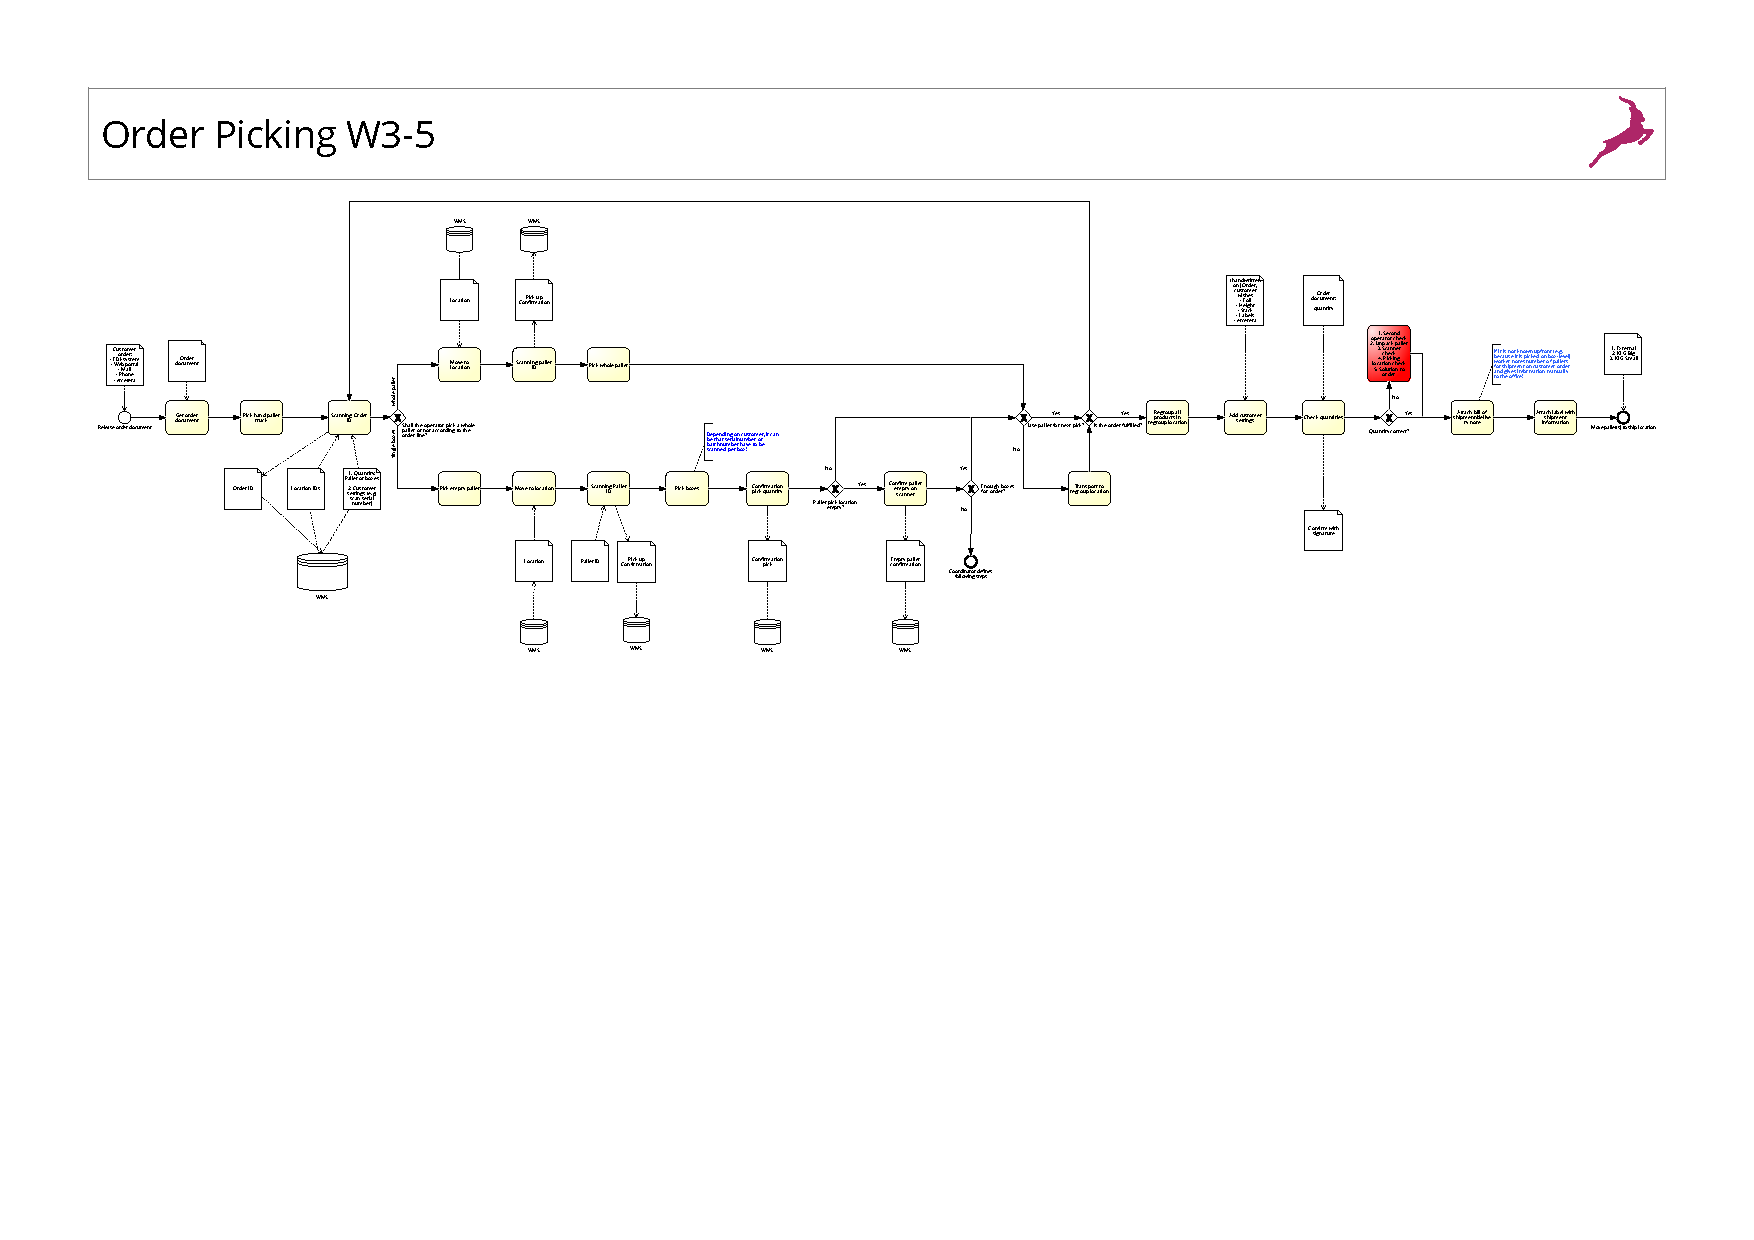
\includegraphics[width=\textwidth, page=1]{images/OrderPickingW3-5}
	\caption{Order Picking Process Diagram \citep{image:logwearOrderPicking}}
	\label{fig:orderPickingProcessDiagram}
\end{figure}
\begin{figure}\ContinuedFloat
	\includegraphics[width=\textwidth, page=2]{images/OrderPickingW3-5}
	\caption*{Figure \ref{fig:orderPickingProcessDiagram}: Order Picking Process Diagram \citep{image:logwearOrderPicking}}
\end{figure}
\begin{figure}\ContinuedFloat
	\includegraphics[width=\textwidth, page=3]{images/OrderPickingW3-5}
	\caption*{Figure \ref{fig:orderPickingProcessDiagram}: Order Picking Process Diagram \citep{image:logwearOrderPicking}}
\end{figure}
\begin{figure}\ContinuedFloat
	\includegraphics[width=\textwidth, page=4]{images/OrderPickingW3-5}
	\caption*{Figure \ref{fig:orderPickingProcessDiagram}: Order Picking Process Diagram \citep{image:logwearOrderPicking}}
\end{figure}
\end{appendices}
\end{document}